\documentclass[12pt,a4paper]{article}
\usepackage[utf8]{inputenc}
\usepackage[russian]{babel}
\usepackage[OT1]{fontenc}
\usepackage{amsmath}
\usepackage{amsfonts}
\usepackage{amssymb}
\usepackage{graphicx}
\usepackage[left=2cm,right=2cm,top=2cm,bottom=2cm]{geometry}
\title{Магнитные моменты легких ядер. Ядерный магнитный резонанс.}
\author{Григорий Чирков}
\begin{document}
\maketitle

\section{Теория}
\subsection{Связь магнитного и механического моментов ядра}

Согласно квантовой механике, полный момент количества движения ядра $\vec{M}$ принимает целые или полуцелые значения (в единицах $\hbar$). Для четного числа нуклонов $M = 0, 1, 2, ... $, а для нечетного $M = 1/2, 3/2, ... $ 

Ядро также обладает магнитным моментом $\vec{\mu}$, связанным с $\vec{M}$. Отношение $\gamma$ магнитного момента к механическому называется гиромагнитным отношением:
\begin{equation}
\vec{\mu} = \gamma \vec{M}.
\end{equation}
Зачастую, вместо $\gamma$ используют более простую величину, $g$-фактор. Он также является отношением магнитного момента к механическому, но при этом магнитный момент измеряется в ядерных магнетонах Бора ($\mu_\text{я} = e \hbar / 2 m_p c$), а механический момент -- в единицах $\hbar$:
\begin{equation}
g = \frac{\mu / \mu _\text{я}}{M/\hbar} = \frac{\mu}{\mu_\text{я}} \frac{\hbar}{M} = \frac{\hbar}{\mu_\text{я}} \gamma.
\end{equation}
Отсюда 
\begin{equation} \label{mu}
\vec{\mu} = \frac{\mu_\text{я}}{\hbar} g \vec{M}.
\end{equation}

Квадрат момента импульса $\vec{M}$ определяется формулой 
\begin{equation}
\vec{M}^2 = \hbar^2 I (I+1),
\end{equation}
где $I$ -- целое или полуцелое число, называемое спином ядра.
\subsection{Магнитный момент ядра}
Проекция момента импульса на любую ось также квантуется. Для проекции момента $\vec{M}$ квантовая механика дает формулу
\begin{equation} \label{Mz}
M_z = m \hbar, 
\end{equation}
где $m$ -- некоторое целое или полуцелое число. Набор всевозможных значений $m$ определяется условием 
\begin{equation}
-I \leq m \leq +I,
\end{equation}
причем последовательные возможные значения $m$ отличаются друг от друга на единицу. Проецируя $M$ и $\mu$ на направление вектора $B$, и применяя формулы (\ref{mu}) и (\ref{Mz}), получаем:
\begin{equation} \label{muB}
\vec{\mu_B} = \frac{\mu_\text{я}}{\hbar} g \vec{M_B} = \mu_\text{я} g m.
\end{equation}
Наибольшее значение $\mu_B$ равно $\mu_\text{я} g I$. Его принято называть магнитным моментом ядра. 

\subsection{Ядро в магнитном поле}
В магнитном поле энергетические уровни ядра расщепляются. Расстояние между двумя соседними компонентами расщепившегося уровня находится с помощью (\ref{muB}):
\begin{equation} \label{deltaE}
\Delta E = B \Delta \mu_B = B \mu_\text{я} g \Delta m = B \mu_\text{я} g.
\end{equation}
\subsection{ЯМР}
Между компонентами расщепившегося уровня могут происходить электромагнитные переходы. Энергия квантов при этом строго определена выражением (\ref{deltaE}), и поэтому явление носит резонансный характер. Частота излучения определяется обычным способом:
\begin{equation} \label{nu}
\nu = \frac{\Delta E}{h} = B \mu_\text{я} g / h.
\end{equation}
Возбуждение переходов между компонентами расщепившегося ядерного уровня носит название ядерного магнитного резонанса (ЯМР). 
\subsection{Измерение $g$-фактора}
В данной работе $g$-фактор определяется с помощью явления ЯМР. Изменяя частоту переменного магнитного поля, мы можем найти положение максимума поглощения, т.е. частоту резонанса. По этому максимуму определяется $g$-фактор из соотношения (\ref{nu}).

\section{Экспериментальная установка}

\begin{figure}[ht!]
 \center{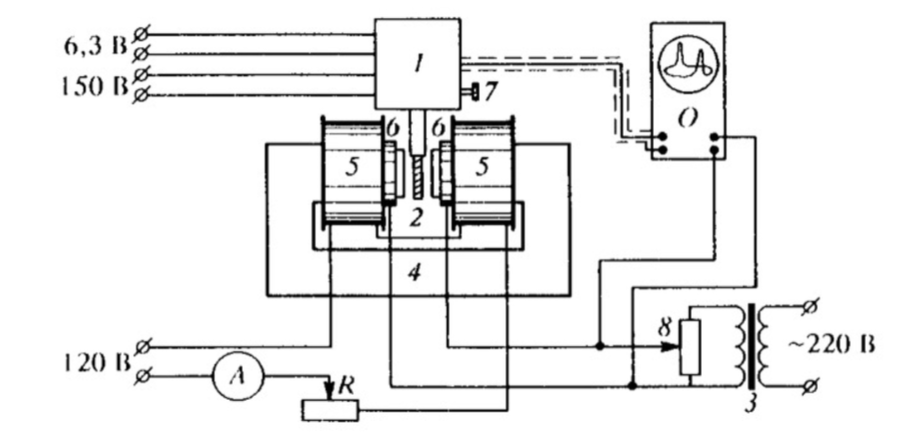
\includegraphics[width=.8\linewidth]{scheme.png}}
\caption{Схема установки}
\end{figure}

Исследуемый образец обозначен цифрой 2. Образец помещен внутрь катушки, входящей в состав генератора. Генератор представляет собой часть индикаторной установки 1. Магнитное поле в образце создается с помощью электромагнита 4. Основное магнитное поле создается с помощью катушек 5, питаемых постоянным током. Величина тока регулируется реостатом $R$ и измеряется амперметром $A$. Небольшое дополнительное поле, генерирующее электромагнитные кванты, возбуждается модулирующими катушками 6, присоединенными к сети переменного тока через трансформатор 3. Напряжение на катушках регулируется потенциометром 8.

\section{Ход работы}

\begin{enumerate}
	\item Для образца с водой:
	\begin{enumerate}
		\item Найти резонанcyю частоту поглощения излучения
		\item С помощью датчика Холла определить магнитное поле в зазоре электромагнита
	\end{enumerate}
	\item Повторить пункты выше для других образцов
\end{enumerate}

\section{Результаты и их обработка}

Все экспериментальные данные и вычисленные значения сведены в таблицу ниже. 

\begin{center}
\begin{tabular}{cccccc}
Вещество 	& $\nu, MHz$	& $B, mT$ 	& $g$-фактор 							& $\mu, \mu_\text{я}$ 	& $\mu_\text{табл}, \mu_\text{я}$ \\
Вода				& $ 9.983 $ 	& $ 230 $  	& $5.7 \pm 0.3 \ (4 \%)$ 		& $2.9 \pm 0.2$			   	& $2.79$ \\
Резина			& $ 10.000 $ 	& $ 230 $ 	& $5.7 \pm 0.3 \ (4 \%)$ 		& $2.9 \pm 0.2$				& $2.79$ \\
Тефлон		& $ 9.990 $   	& $ 250 $ 	& $5.3 \pm 0.2 \ (4 \%)$ 		& $2.7 \pm 0.1$				& $2.63 $ \\
Дейтерий		& $ 3.481 $		& $ 530 $ 	& $0.86 \pm 0.02 \ (2 \%)$ 	& $0.86 \pm 0.02$			& $0.857$ \\ 
\end{tabular}
\end{center}

Расчет $g$-фактора сделан по формуле 
\begin{equation}
g_\text{я} = \frac{h \nu}{\mu_\text{я} B}, 
\end{equation}
а магнитного момента -- по формуле (\ref{muB}). При подсчете погрешностей учтено, что $\sigma_B = 10 mT, \sigma_\nu = 1kHz$. Все табличные данные взяты из справочника физических величин(под ред. И.К. Кикоина).

\section{Вывод}

В проделанном эксперименте было изучено явление ядерно-магнитного резонанса. В ходе работы была получена осциллограмма резонансной кривой, резонансные значения магнитного поля и частоты внешнего излучения. На основе полученных данных были расчитаны $g$-факторы и магнитные моменты ядер водорода, дейтерия и фтора. Все полученные значения сходятся с табличными в пределах погрешности.


\end{document}